\documentclass[12pt]{article}
  \usepackage[francais]{babel}
  \AddThinSpaceBeforeFootnotes % à insérer si on utilise \usepackage[french]{babel}
  \FrenchFootnotes % à insérer si on utilise \usepackage[french]{babel}
  \usepackage[T1]{fontenc}
  \usepackage[utf8]{inputenc}
  \usepackage{graphicx}
  \usepackage[left=2.5cm,right=2.5cm,top=2.5cm,bottom=2.5cm]{geometry}
  \usepackage{array}
  \usepackage{booktabs}
  \usepackage[squaren,Gray]{SIunits}  % Unité ex: $\unit{5 \cdot 10^{-6}}{\meter}$
  \usepackage{colortbl}               % Pour les couleur des cellules (tableau)
  \usepackage{amsmath}				  % Pour les formules mathématiques
  \usepackage{upgreek}                % Pour les lettres greque
  %\usepackage{fullpage}	          % plus petites marges
  \usepackage{verbatim}				  % Pour de long commentaires
  \usepackage[lofdepth,lotdepth]{subfig}       % Faire des sous-figures
  \usepackage{url}
  \usepackage{colortbl}               % pour les couleur des cellules (tableau)
  \usepackage{indentfirst}
  \usepackage{multirow}
  \usepackage{xfrac}
  \usepackage{wrapfig}
  \usepackage{enumitem}               % Liste personnalisée
  \frenchbsetup{StandardLists=true}   % Empêche conflits entre enumitem et babel
  \usepackage{placeins}   % place une barrière pour que l'image/table soit derrière \FloatBarrier
  \usepackage{lastpage} 
  \usepackage{titling}
  \usepackage{lmodern}
  \usepackage{booktabs}
  \usepackage{etoolbox}
  \usepackage[most]{tcolorbox}
  
  
  %Change la taille de police
  \newcommand\ChangeRT[1]{\noalign{\hrule height #1}}
  
\graphicspath{{images/}}

  
  %Création  d'une nouvelle commande pour faire référence à une Figure
  %Exemple : \appelFigure{schema} donne : Figure 1 (en italique)
  \newcommand{\appelFigure}[1]{
    \textit{Figure \ref{#1}}
  }
      
  %%Création commande pour insérer image avec nom de figure directement
  %\newcommand{nomDeTaCommande}[nombreArguments]{CodeLaTeX}
  %\insertImage[position]{image_path}{scale}{Titre_figure}{label}
  \newcommand{\insertImage}[5][center]{
      \begin{#1}
      \includegraphics[scale=#3]{#2}
      \captionof{figure}{#4} 
      \label{#5}
      \end{#1}
  }

  % Affichage des frames pour commande cisco
  \newtcblisting{cisco}[1][]{size=fbox, listing only, listing options={style=tcblatex,basicstyle=\ttfamily\scriptsize,tabsize=2,language=sh},title=#1}

  %En-tête et pied de page personalisé
  \usepackage{fancyhdr}
  \pagestyle{fancy}
  \fancyhf{}
  \setlength\parindent{0pt} %Supprime les alinéa
  \setlength{\parskip}{8pt} %Augmente l'espace entre paragraphe
  %Bottom numbering page
  \renewcommand{\headrulewidth}{1pt}
  \fancyhead[L]{
\includegraphics[scale=.2]{heia-fr-logo.png}}
  \fancyhead[R]{\theauthor}
  
  \renewcommand{\footrulewidth}{1pt}
  \fancyfoot[R]{\textbf{Page \thepage\ sur \pageref{LastPage}}} 
%  \fancyfoot[L]{\leftmark}

  \setlength\parindent{0pt} %Supprime les alinéa
  \setlength{\parskip}{8pt} %Augmente l'espace entre paragraphe


\title{Système Embarqués II, Journal, TP.02:\\ Introduction à la programmation modulaire en C} 
\author{\textsl{Marc} \textsc{Roten} \\ \textsl{Sven} \textsc{Rouvinez}}
\date{}

\begin{document}
    \begin{titlepage}
        \begin{center}
            
\includegraphics[scale=.3]{heia-fr-logo.png}\\[1.3cm]
            
            \rule{\linewidth}{0.3mm} \\[0.3cm]
            {\huge \bfseries Système embarqués \\[0.5cm]} 
           % {\Large Effet photoélectrique}\\[0.2cm]
            \rule{\linewidth}{0.3mm} \\[0.8cm]
            \noindent
            \begin{minipage}[t]{0.4\textwidth}
                \begin{flushleft} \large
                    \emph{Auteurs :}\\
                    \theauthor
                \end{flushleft}
            \end{minipage}
            \begin{minipage}[t]{0.4\textwidth} 
                \begin{flushright} \large
                    \emph{Professeur:}\\
                    \textsl{Daniel} \textsc{Gachet}\\ 
                \end{flushright} 
                \vfill
            \end{minipage}\\[1.3cm]
            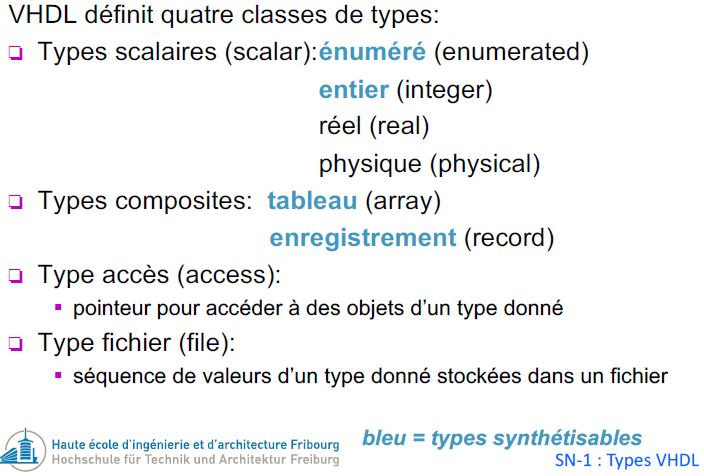
\includegraphics[scale=0.6]{1.JPG}\\[1.5cm]
            \vspace*{1\baselineskip}
            \today \\[0.7cm]
        \end{center}
    \end{titlepage}
    \tableofcontents
    \clearpage
% \insertImage{Img/1.PNG}{echelle pour l'image (source = 1)}{texte dessous l'image}{référence vers l'objet}

\section{Pourrait-on se passer des fichiers d'entête (header files) en C ?} 
Oui il est possible de se passer des fichiers d'entête, il suffirait de mettre les signatures dans les fichiers source tout en haut

\section{\#pragma once}
Il permet d'éviter un import multiple de header files et peut être accompagné des commandes preprocessor \texttt{\#ifndef symbol \#define}


\section{Que faut-il placer dans un fichier d'entête ?}
Il faut placer la signature des méthodes qui sont utilisées dans le fichier source

\section{Quelle est l'utilité des mots-clef extern et static ?}
Le mot-clé \texttt{extern} permet de déclarer une variable à l'extérieur d'un fichier source pour qu'elle soit accessible par les autres fichiers sources\\
\texttt{static} définit le scope où la variable est accessible uniquement dans la classe ou dans la méthode qui l'utilise

\section{Comment faut-il procéder pour définir une constante en C ?}
\begin{itemize}
   \item \texttt{const type nom\_variable=valeur}
   \item \texttt{\#define NOM valeur}
\end{itemize}

\section{Quelle(s) différence(s) existe-t-il entre les instructions}
\begin{enumerate}
   \item   \#define MAX 10
   \item const int MAX=10
\end{enumerate}
La première est une commande preprocesseur et donc partout où l'on va utiliser MAX il sera remplacé par 10 et l'autre est une variable qui est constante donc elle a un type 


\section{Comment peut-on définir une énumération en C ? Quelle est son utilité ?}
\texttt{enum colors \{RED, YELLOW, BLUE\}} et permet d'initialiser une séquence de constantes qui pourra être utilisé plus tard

\section{Quelle(s) différence(s) existe-t-il entre une structure en C struct S\{\} et une classe en Java class C\{\} ?}
\texttt{struct S\{\}} permet de définir une structure par exemple un tableau avec plusieurs champ et chaque champ a un nom\\
\texttt{class C\{\}} permet de déclarer une class

\section{Comment faut-il procéder pour définir un tableau en C ? Peut-on lui donner des valeurs initiales lors de sa définition ?}
\texttt{int array\_declaration[10];} et avec l'affectation \texttt{int array\_declaration[]=\{10,9,8,7\};}

\section{Comment faut-il procéder pour obtenir le nombre d'éléments contenus dans un tableau ?}
\texttt{sizeof(array)/sizeof(array[0])}\\ \texttt{sizeof} retourne la taille de l'objet que l'on divise par le taille du type contenu
\end{document}
